\documentclass[sigconf,nonacm]{acmart}
\settopmatter{printacmref=false,printfolios=true}
\renewcommand\footnotetextcopyrightpermission[1]{}
\pagestyle{plain}

\usepackage{booktabs}
\usepackage{array}
\usepackage{tikz}
\usetikzlibrary{arrows.meta,positioning,fit,calc}

\begin{document}

\title{Can eBPF Run a Real Language Model?}
\subtitle{Lessons from a Kernel-Resident Qwen3 Forward Pass}

\author{Yusheng Zheng}
\affiliation{%
  \institution{UC Santa Cruz}
  \city{Santa Cruz}
  \state{CA}
  \country{USA}}
\email{yzhen165@ucsc.edu}

\begin{abstract}
eBPF programs usually observe or steer work that happens elsewhere in the
kernel. We ask a different question: can verifier-checked BPF code do the
arithmetic of a real language model, and what does that cost? bpfllm runs the
complete forward pass of Qwen3-0.6B, from the first decoder layer to the
151,936-token vocabulary projection, in BPF programs that the stock
Linux~6.17 verifier accepts, with no kernel module. In its event-driven mode,
a UDP packet that reaches XDP starts the computation, BPF code walks all 28
layers over BF16 weights held in a BPF arena, and the next token goes back in
an XDP reply. No user-space thread takes part after loading. Accuracy holds
up: integer fixed-point arithmetic chose the same next token as the official
BF16 model at 251 of 256 positions in two text excerpts, and four of the five
differences were ties. Speed does not. Batching cut kernel crossings 34-fold,
to 4,169 per token, and in-kernel scheduling produced one token in 580\,ms,
yet on 125- and 131-token sequences the kernel path was 1.8--4.8$\times$
slower than ordinary BF16 inference on one CPU core. The verifier shaped the
code but never stopped it; the limit was the BPF instruction set, which has
no floating point or vector instructions. We describe how the model got
through the verifier and what this means for machine learning inside the
kernel.
\end{abstract}

\maketitle

\section{Introduction}

Most eBPF programs are small: they trace a system call, filter a packet or
make a scheduling decision. Kernel policies for congestion control,
scheduling and storage have started to use learned models, but the models
placed in the kernel have stayed small as well. They are decision trees and
compact quantized networks, run in kernel modules, in eBPF or on a
GPU~\cite{liteflow,lake,kml,bachl}. Two questions remain open: how far
verified BPF code can go on its own, and which limit binds first, the
verifier, the instruction set or the execution model.

We take these questions to an extreme by running a real language model,
Qwen3-0.6B~\cite{qwen3}, in eBPF. The goal is not to serve LLMs from the
kernel. A modern transformer uses every kind of operator at once (large
matrix products, normalization with square roots, transcendental
activations, softmax, rotary position embeddings and a growing cache), and it
presses against every resource limit of BPF. That makes it a good probe of
what the kernel extension model can express and what it costs. This paper
contributes:

\begin{itemize}
\item bpfllm, a complete Qwen3-0.6B forward pass in Linux eBPF with two
modes. In \emph{operator mode}, a C driver calls six bounded BPF operators.
In \emph{event mode}, a packet triggers all 28 layers, the KV-cache update,
the vocabulary argmax and the UDP reply inside BPF, with no user-space
involvement after loading (\S\ref{sec:design}). A September 2026 search found
no other public full Qwen3-0.6B forward pass in Linux eBPF;
\item the techniques that got the model past the verifier: per-tensor
fixed-point formats, bounded \texttt{bpf\_loop} batches, lookup tables and a
work item that requeues itself one step at a time (\S\ref{sec:verifier});
\item a comparison of output fidelity against the official BF16 model, and an
analysis of where the time goes (\S\ref{sec:eval});
\item lessons for placing machine learning inside the kernel
(\S\ref{sec:lessons}).
\end{itemize}

\section{Constraints and Target}
\label{sec:background}

\paragraph{What BPF provides.} BPF has a 64-bit integer instruction set with
no floating point and no vector instructions. Before a program loads, the
verifier proves that it is memory safe and terminates by exploring its
paths, within a budget of one million processed
instructions~\cite{verifierdoc}. Loops must be bounded; the
\texttt{bpf\_loop} helper~\cite{bpfloop} runs a callback a bounded number of
times while verifying it only once. Data lives in maps. Array maps can be
memory-mapped into user space, and BPF arenas~\cite{arena} (Linux~6.9) give
BPF and user space a large shared region addressed by pointers. A program
can run synchronously from a system call through \texttt{BPF\_PROG\_RUN}, per
packet in softirq context at XDP~\cite{xdp}, where it must finish quickly, or
later in a kernel worker through a BPF workqueue~\cite{bpfwq} (Linux~6.10).

\paragraph{The model.} Qwen3-0.6B has 28 decoder layers and a hidden width of
1,024. Each layer has 16 query heads and 8 key/value heads of dimension 128,
and an MLP of width 3,072. The 151,936-token vocabulary projection reuses the
embedding matrix. By our count, one token needs about 596 million
multiply-accumulates (MACs), 26\% of them in the vocabulary projection. The
official BF16 weight file is 1.5\,GB.

\section{Design}
\label{sec:design}

\subsection{Integer arithmetic}

Since BPF has no floating point, every tensor is stored in fixed point: a
Q$n$ value is a real number scaled by $2^n$ and kept as an integer.
Activations use Q16, matrix weights Q24 and normalization scales Q20,
because some official norm weights are too large for Q24 in 32 bits.
Products accumulate in 64 bits. RMSNorm uses an integer square root, SiLU an
integer approximation (maximum error 0.000634 on $[-8,8]$), and attention an
online, numerically stable integer softmax (maximum output error 0.000905 in
synthetic tests of up to 257 positions). Precision matters more than it first
seems. On one official projection row, Q8 weights gave $-0.0367$ against a
BF16 result of $-0.00837$, because large terms cancel; Q24 gave $-0.00838$.

\subsection{Operator mode}

Six BPF programs implement the model: batched matrix rows, RMSNorm, RoPE,
attention, SiLU and elementwise vector operations. They are declared as
socket-filter programs, but the C driver never attaches them to a socket; it
runs each one directly through \texttt{BPF\_PROG\_RUN}. For each step, the
driver takes the needed rows from the memory-mapped BF16 weight file,
converts them to Q24, writes them with the activations into a memory-mapped
work map, runs the operator and reads back the result. One call handles up to
128 matrix rows, all 24 query and key heads for normalization or RoPE, a
whole 3,072-element vector, or 256 positions of attention history. The
attention program owns the KV cache: it writes each new key and value into a
BPF array map and scans the history in bounded chunks. During the vocabulary
projection, the matrix callback also tracks the running argmax. One token
costs 4,169 \texttt{bpf()} system calls. An optional variant copies the whole
BF16 payload into BPF arena pages once; BPF then reads rows at their file
offsets and converts them through a 65,536-entry BF16-to-Q24 lookup table.
It produces byte-identical logits.

\subsection{Event mode}

\begin{figure}[t]
\centering
\resizebox{\columnwidth}{!}{%
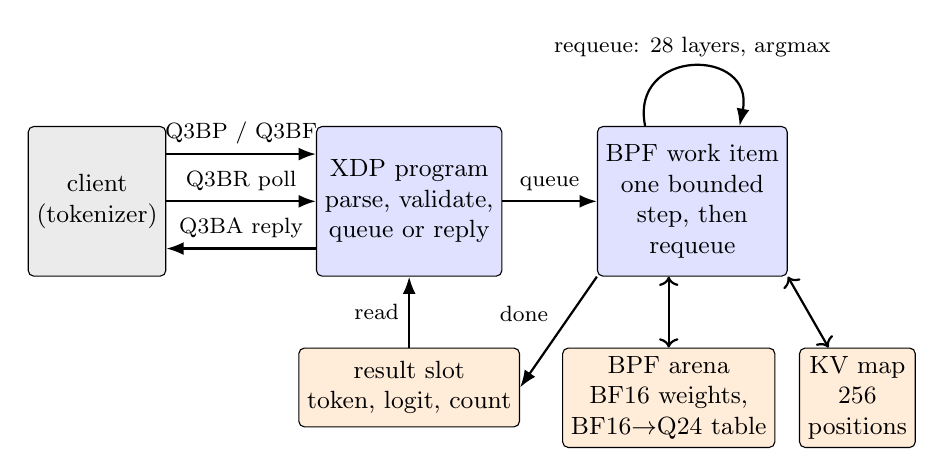
\begin{tikzpicture}[
  font=\small,
  box/.style={draw,rounded corners=2pt,align=center,minimum height=10mm,inner sep=3pt},
  bpf/.style={box,fill=blue!12},
  mem/.style={box,fill=orange!15},
  usr/.style={box,fill=black!8},
  arr/.style={-{Latex[length=2.2mm]},thick}]
\node[usr,minimum height=19mm] (cl) {client\\(tokenizer)};
\node[bpf,minimum height=19mm,right=19mm of cl] (xdp) {XDP program\\parse, validate,\\queue or reply};
\node[bpf,minimum height=19mm,right=12mm of xdp] (wq) {BPF work item\\one bounded\\step, then\\requeue};
\node[mem,below=9mm of xdp] (res) {result slot\\token, logit, count};
\node[mem,below=9mm of wq,xshift=-3mm] (ar) {BPF arena\\BF16 weights,\\BF16$\to$Q24 table};
\node[mem,right=3mm of ar] (kv) {KV map\\256\\positions};
\draw[arr] ([yshift=6mm]cl.east) -- node[above,font=\footnotesize]{Q3BP / Q3BF} ([yshift=6mm]xdp.west);
\draw[arr] ([yshift=0mm]cl.east) -- node[above,font=\footnotesize]{Q3BR poll} ([yshift=0mm]xdp.west);
\draw[arr] ([yshift=-6mm]xdp.west) -- node[above,font=\footnotesize]{Q3BA reply} ([yshift=-6mm]cl.east);
\draw[arr] (xdp) -- node[above,font=\footnotesize]{queue} (wq);
\draw[arr] ([xshift=-6mm]wq.north) .. controls +(-0.2,1.0) and +(0.2,1.0) .. node[above,font=\footnotesize]{requeue: 28 layers, argmax} ([xshift=6mm]wq.north);
\draw[arr,<->] ([xshift=-3mm]wq.south) -- (ar);
\draw[arr,<->] (wq.south east) -- (kv);
\draw[arr] (wq.south west) -- node[above left,font=\footnotesize]{done} (res.east);
\draw[arr] (res) -- node[left,font=\footnotesize]{read} (xdp);
\end{tikzpicture}}
\caption{Event mode. Blue boxes are BPF programs and orange boxes are BPF
memory. After loading, the user-space loader only holds the XDP link; the
client tokenizes text and sends token IDs but does no model arithmetic.}
\label{fig:event}
\end{figure}

Operator mode still schedules the 28 layers from user space. Event mode moves
that schedule into the kernel (Figure~\ref{fig:event}). At startup, a loader
maps the model, copies its complete BF16 payload into a BPF arena, records
where each layer's tensors start, initializes a BPF workqueue and attaches an
XDP program to a UDP port. From then on it only keeps the XDP link alive.

Each request packet carries a token ID and its position. A \texttt{Q3BP}
request asks for the next token; a \texttt{Q3BF} request only extends the
context and skips the vocabulary projection, which makes prompt prefill
cheaper. The XDP program checks the magic value, the token range and that
positions arrive in order, and then queues the work item. It never computes
inline: one token takes hundreds of milliseconds, and XDP runs in softirq
context. The work item is a state machine. Each time it runs, it performs one
bounded step (a 128-row matrix batch, a normalization, an attention chunk,
SiLU or a residual add) and requeues itself, until the token is finished. It
reads the embedding, all weights and the RoPE inverse frequencies from the
arena and computes the RoPE coefficients itself. Keys and values go into a
layer-indexed KV map with 256 positions for a single session. After layer 28,
the work item applies the final norm and runs all 151,936 vocabulary rows
with a fused argmax.

The computation outlives the request packet, so the client polls for the
answer with a \texttt{Q3BR} packet carrying the expected completion count.
When the count matches, XDP rewrites the poll into a 20-byte \texttt{Q3BA}
reply holding the token ID, its Q16 logit and the count, swaps the addresses
and ports, and sends it back with \texttt{XDP\_TX}. Polls that arrive early or
carry a stale count are dropped. An earlier version passed them up to the
network stack, which answered with ICMP ``port unreachable'' messages.

\subsection{Getting through the verifier}
\label{sec:verifier}

The verifier rejected two natural designs, and both had simple fixes. A
single RMSNorm program exceeded the one-million-instruction budget. Splitting
it into two \texttt{bpf\_loop} callbacks, one that accumulates and one that
applies the scale, with an integer square root in between, let it load.
Converting BF16 to Q24 inside the 3,072-column loop failed with ``The
sequence of 8193 jumps is too complex''; a 65,536-entry lookup table indexed
by the BF16 bit pattern replaced the branches with a single load. More
generally, we sized every unit of work so that a callback is verified once
and runs for a bounded time. That is also the granularity the workqueue state
machine needs.

Correctness came from differential testing. We compared each operator, and in
event mode every prefix of two to 28 layers, element by element against an
independent C implementation of the same fixed-point arithmetic. The
comparison even caught a signed/unsigned multiplication bug in the C
reference itself, which first showed up at layer four.

\section{Evaluation}
\label{sec:eval}

\paragraph{Setup.} We ran on an arm64 host with Cortex-X925 and Cortex-A725
cores under Linux 6.17.0-1029-nvidia, using an Ubuntu 24.04 build container,
Clang~19 and libbpf~1.7. We use the official Qwen3-0.6B weights and
tokenizer; the artifact records their hashes. The reference is the official
model running in Transformers 5.14.1 and PyTorch 2.11.0 on the CPU. The host
was shared and not isolated, so we report single runs or medians of three,
all measured after the model was loaded, and treat timings as exploratory.
Where noted, processes are pinned to one core; on this heterogeneous CPU,
unpinned workqueue placement changed latency by about 2$\times$.

\subsection{Fidelity}

\begin{table}[t]
\centering
\small
\caption{Agreement with the official BF16 model. MAE is the mean absolute
error over all 151,936 logits. The sequence rows compare the argmax at each
prefix with an incremental BF16 run that uses a KV cache.}
\label{tab:fidelity}
\begin{tabular}{@{}>{\raggedright\arraybackslash}p{0.36\columnwidth}>{\raggedright\arraybackslash}p{0.38\columnwidth}r@{}}
\toprule
Input & Agreement & MAE \\
\midrule
Token 0 / token 1 & next ID 9 / 14582, top 3 & 0.052 / 0.030 \\
{[0, 1]}, then one decode step & IDs 220, 16, top 3 & 0.024 / 0.025 \\
{[0, 1, 2, 3]} & next ID 2, top 4 & 0.019 \\
``Hello, world!'' & next ID 1096, top 5 & 0.035 \\
\midrule
131-token test file & argmax 128 of 131 & -- \\
WikiText-2 row 1011 & argmax 123 of 125 & -- \\
\midrule
WikiText-2 rows 3--4 & perplexity 24.82 vs.\ 24.01 & -- \\
WikiText-2 row 1011 & perplexity 17.22 vs.\ 15.88 & -- \\
\bottomrule
\end{tabular}
\end{table}

Table~\ref{tab:fidelity} shows that fixed-point inference picks the same next
token as BF16 for every short input, with logit errors of 0.019--0.052. On
two longer sequences, a 131-token test file and a 125-token
WikiText-2~\cite{wikitext} excerpt, event mode matched the BF16 argmax at 251
of 256 prefixes. Four of the five mismatches were exact ties in BF16. In the
fifth, bpfllm chose the BF16 runner-up, 0.125 logit below the winner;
operator mode made the same choice, so event scheduling is not the cause.
With teacher forcing, perplexity on two WikiText-2 excerpts was 3.4\% and
8.4\% higher than BF16. Event and operator mode chose the same token at every
prefix of a 131-token input. Their logits first differed at position 36,
where the in-BPF integer RoPE cosine is one Q20 unit away from the C driver's
libm value, and they never differed by more than 0.005.

Lower precision failed this test. A naive group-wise INT4 format shrank the
matrices to 317\,MB including scales and cut forward time by 23\% (0.956
versus 1.243\,s), but it changed the next token for all three inputs we
tried, for example from ID 9 to 284, with a logit MAE of 0.98--1.84. Finer
groups, a Q24 vocabulary projection or quantizing only the MLP did not bring
the right token back. A group-32 INT8 format changed the prediction for
``Hello, world!''; per-row int16 kept the top token but ran at half the
speed; and converting all matrices to Q24 ahead of time doubled the file to
3.0\,GB and ran slower.

\subsection{Where the time goes}

\begin{table}[t]
\centering
\small
\caption{Kernel crossings and one-token time in operator mode. Times are
medians of three interleaved runs, except single runs ($^s$) and one
non-interleaved median ($^n$).}
\label{tab:crossings}
\begin{tabular}{@{}>{\raggedright\arraybackslash}p{0.42\columnwidth}rr@{}}
\toprule
Change & \texttt{bpf()} calls & Time (s) \\
\midrule
Map weight file instead of reading it & 143,667 & 2.91$\to$2.70$^s$ \\
4$\to$16 rows per matrix call & $\to$50,667 & 2.70$\to$1.61$^s$ \\
One call per RMSNorm & $\to$43,171 & 1.20$\to$1.28 \\
128 rows, fused argmax, batched vectors, RoPE, SiLU & $\to$5,229 & -- \\
All Q/K norm heads per call & $\to$4,587 & 1.20$\to$1.21 \\
All query heads per attention chunk & $\to$4,169 & 1.02$^n$ \\
\midrule
BF16$\to$Q24 by table lookup & unchanged & 1.48$\to$1.15 \\
\bottomrule
\end{tabular}
\end{table}

Early versions crossed the user/kernel boundary hundreds of thousands of
times per token (Table~\ref{tab:crossings}). Before the weight file was
memory-mapped, each token also made 788,197 \texttt{lseek} and \texttt{read}
calls. Mapping the file and doing more work per call helped at first: going
from 4 to 16 rows per matrix call cut \texttt{bpf()} calls 2.8$\times$ and
time from 2.70 to 1.61\,s. A further 12$\times$ reduction, from 50,667 to
4,169 calls, left one-token time between 1.0 and 1.3\,s, within run-to-run
noise. By contrast, replacing per-weight conversion arithmetic with a table
lookup, which changes no crossings at all, cut time from 1.48 to 1.15\,s.
Below roughly 50,000 crossings per token, arithmetic dominates.

That arithmetic is slow. By our count, event mode sustained about 1.0 billion
MACs per second for one token, while BF16 PyTorch on one core sustained
2.9--4.1 billion over a 131-token run. Each BPF MAC is a chain of scalar
instructions: load a BF16 value from the arena, look up its Q24 value,
multiply in 64 bits and add. The model reads about 1.2\,GB of weights per
token, or about 2\,GB/s at 580\,ms, far below what the memory system
delivers, so the loop is limited by instructions rather than by bandwidth.
Splitting the dot product into two independent accumulators cut a 131-token
run by 6.5\% (median 93.2 to 87.1\,s), which also points to instruction
latency.

\subsection{Kernel scheduling versus user space}

\begin{table}[t]
\centering
\small
\caption{Latency after model loading. Event: XDP-triggered, no user-space
dispatch. Operator: arena variant dispatched by C. BF16: official model in
PyTorch on one core with a KV cache. Ranges span repeated runs.}
\label{tab:latency}
\begin{tabular}{@{}lrrr@{}}
\toprule
Workload & Event & Operator & BF16 \\
\midrule
1 token, X925 core & 0.58\,s & 0.81\,s & -- \\
1 token, A725 core & 1.22\,s & 1.86\,s & -- \\
10 tokens & 5.71\,s & 4.78--5.71\,s & -- \\
131-token prompt, prefill$^a$ & 61.0\,s & 57.6\,s & -- \\
131 tokens, all logits & 88.8--93.2\,s & -- & 19.2--26.9\,s \\
125 tokens, all logits & 85.2\,s & -- & 43.9--46.2\,s \\
\bottomrule
\multicolumn{4}{@{}l}{\footnotesize $^a$Median of three; only the last
position computes vocabulary logits.}
\end{tabular}
\end{table}

Event mode removes every user-space dispatch. For one token on a pinned core,
its latency was 29\% lower than the operator-mode arena driver on a
Cortex-X925 core and 34\% lower on a Cortex-A725 core
(Table~\ref{tab:latency}). The advantage did not carry over to sequences:
over ten tokens and over a 131-token prompt, event mode was no faster.
Per-token poll round trips and workqueue placement, which these standalone
runs did not record, may contribute. Against the conventional baseline the
picture is clear. Computing logits at every position, event mode was
1.8--4.8$\times$ slower than BF16 on one core. Normal inference practice
widens the gap further: a batched four-core BF16 pass, which processes all
positions of a prompt at once, scored a 423-token excerpt in 6.4\,s, while
operator mode, scoring one position at a time, took 401.6\,s.

\section{Lessons}
\label{sec:lessons}

\emph{The verifier shapes the code but is not a wall.} Every rejection we hit
was fixed by restructuring the work into bounded callbacks or by turning
branches into table lookups. A full transformer, including softmax, square
roots and a KV cache, fits in verified BPF on a stock kernel.

\emph{Reduce crossings first, then stop.} Cutting kernel crossings was the
right first optimization, but its returns vanished below about 50,000 per
token. Removing user-space scheduling entirely made single tokens a third
faster, yet still did not beat user-space inference.

\emph{The instruction set sets the ceiling.} Without floating point or vector
instructions, every weight costs several scalar instructions, and one
ordinary user-space core stayed 1.8--4.8$\times$ faster. Closing that gap
would need dense-math support in BPF itself, such as vector instructions or
verified kfuncs for matrix kernels. How to offer either without weakening the
verifier's guarantees is an open question.

\emph{Fixed point is enough for argmax; naive low-bit formats are not.} Q24
weights kept the model's choices nearly intact, while the faster INT4 variant
changed them. Calibrated schemes such as GPTQ~\cite{gptq} or AWQ~\cite{awq}
would need whole-model token and logit checks before adoption.

\emph{The event structure is reusable.} XDP to admit and queue a request, a
self-requeuing work item to compute, and a poll answered with
\texttt{XDP\_TX} together form a complete request path with no user-space
worker. It suits a small model that makes one decision per packet or per
kernel event far better than it suits LLM serving.

\section{Related Work}

\emph{Machine learning in the kernel.} LiteFlow~\cite{liteflow} runs
quantized neural network snapshots in the kernel datapath, LAKE~\cite{lake}
offloads kernel ML to GPUs, KML~\cite{kml} brings a small ML framework into
the kernel for storage tuning, and Bachl et al.~\cite{bachl} run decision
trees for intrusion detection in eBPF. Their models are orders of magnitude
smaller than ours. KernelX~\cite{kernelx} takes the opposite placement: it
feeds eBPF signals to an LLM running in user space.

\emph{Small inference engines and integer inference.} Single-file C engines
such as qwen3.c~\cite{qwen3c} show how compact a Qwen3 forward pass can be on
a CPU. Integer-only inference~\cite{jacob} and integer approximations of
softmax and normalization for transformers~\cite{ibert} motivate our
fixed-point operators.

\emph{BPF mechanisms.} Our design depends on bounded batching with
\texttt{bpf\_loop}~\cite{bpfloop}, resident weights in BPF
arenas~\cite{arena}, deferred computation in BPF workqueues~\cite{bpfwq}, and
XDP~\cite{xdp} for the request path. Verifier analyses such as
PREVAIL~\cite{prevail} study the limits that shaped our operators.

\section{Limitations and Conclusion}

All results come from one shared arm64 host running Linux~6.17, mostly single
runs or medians of three. Fidelity covers a handful of short inputs and two
text excerpts, not a benchmark. Event mode serves one session with a
256-position cache and needs a fresh loader for each sequence. Its dense KV
layout costs 224\,KiB per position, so the model's 40,960-position context
is out of reach here. Other kernels and architectures would need their own
verifier validation, and the prototype must not run on production kernels.

A real language model can run inside Linux eBPF, from packet to token, with
accuracy close to BF16. It runs slower than one ordinary CPU core, and the
reason is the arithmetic the BPF instruction set offers, not the verifier or
the user/kernel boundary. Source code, commands and all recorded
measurements are at \url{https://github.com/eunomia-bpf/qwen3-ebpf} (MIT
license).

\begin{thebibliography}{99}
\bibitem{liteflow} J.~Zhang, C.~Zeng, H.~Zhang, S.~Hu, K.~Chen. LiteFlow:
Towards High-Performance Adaptive Neural Networks for Kernel Datapath.
SIGCOMM 2022.
\bibitem{lake} H.~Fingler et al. Towards a Machine Learning-Assisted Kernel
with LAKE. ASPLOS 2023.
\bibitem{kml} I.~U.~Akgun et al. KML: Using Machine Learning to Improve
Storage Systems. arXiv:2111.11554, 2021.
\bibitem{bachl} M.~Bachl, J.~Fabini, T.~Zseby. A Flow-based IDS Using Machine
Learning in eBPF. arXiv:2102.09980, 2021.
\bibitem{qwen3} A.~Yang et al. Qwen3 Technical Report. arXiv:2505.09388,
2025.
\bibitem{verifierdoc} Linux kernel documentation. eBPF verifier.
\url{https://docs.kernel.org/bpf/verifier.html}.
\bibitem{prevail} E.~Gershuni et al. Simple and Precise Static Analysis of
Untrusted Linux Kernel Extensions. PLDI 2019.
\bibitem{bpfloop} J.~Koong. bpf: Add bpf\_loop helper. Linux~5.17, 2021.
\bibitem{arena} A.~Starovoitov. bpf: Introduce BPF arena. Linux~6.9, 2024.
\bibitem{bpfwq} B.~Tissoires. BPF workqueues (bpf\_wq). Linux~6.10, 2024.
\bibitem{xdp} T.~H{\o}iland-J{\o}rgensen et al. The eXpress Data Path: Fast
Programmable Packet Processing in the Operating System Kernel. CoNEXT 2018.
\bibitem{wikitext} S.~Merity, C.~Xiong, J.~Bradbury, R.~Socher. Pointer
Sentinel Mixture Models. ICLR 2017.
\bibitem{gptq} E.~Frantar, S.~Ashkboos, T.~Hoefler, D.~Alistarh. GPTQ:
Accurate Post-Training Quantization for Generative Pre-trained Transformers.
ICLR 2023.
\bibitem{awq} J.~Lin et al. AWQ: Activation-aware Weight Quantization for
On-Device LLM Compression and Acceleration. MLSys 2024.
\bibitem{kernelx} KernelX: an eBPF bridge to a user-space LLM.
\url{https://github.com/pie-314/KernelX}.
\bibitem{qwen3c} A.~Cable. qwen3.c: Qwen3 inference in pure C.
\url{https://github.com/adriancable/qwen3.c}.
\bibitem{jacob} B.~Jacob et al. Quantization and Training of Neural Networks
for Efficient Integer-Arithmetic-Only Inference. CVPR 2018.
\bibitem{ibert} S.~Kim, A.~Gholami, Z.~Yao, M.~W.~Mahoney, K.~Keutzer. I-BERT:
Integer-only BERT Quantization. ICML 2021.
\end{thebibliography}

\end{document}
